\documentclass[nobib]{tufte-handout}
\usepackage[utf8]{inputenc}
\usepackage[estonian]{babel}
\usepackage[style=english]{csquotes}

\title{IDU1321 - Ettevõtte äriarhitektuur. Iseseisev töö}
\author[Andres Kütt]{Andres Kütt}

%\date{04.08.2017}
%\geometry{showframe} % debug

\usepackage{natbib}

\usepackage{graphicx}
 \setkeys{Gin}{width=\linewidth,totalheight=\textheight,keepaspectratio}
  \graphicspath{{graphics/}} % set of paths to search for images
\usepackage{amsmath}  % extended mathematics
\usepackage{booktabs} % book-quality tables
\usepackage{units}    % non-stacked fractions and better unit spacing
\usepackage{multicol} % multiple column layout facilities
\usepackage{lipsum}   % filler text
\usepackage{fancyvrb} % extended verbatim environments
  \fvset{fontsize=\normalsize}% default font size for fancy-verbatim environments

% Standardize command font styles and environments
\newcommand{\doccmd}[1]{\texttt{\textbackslash#1}}% command name -- adds backslash automatically
\newcommand{\docopt}[1]{\ensuremath{\langle}\textrm{\textit{#1}}\ensuremath{\rangle}}% optional command argument
\newcommand{\docarg}[1]{\textrm{\textit{#1}}}% (required) command argument
\newcommand{\docenv}[1]{\textsf{#1}}% environment name
\newcommand{\docpkg}[1]{\texttt{#1}}% package name
\newcommand{\doccls}[1]{\texttt{#1}}% document class name
\newcommand{\docclsopt}[1]{\texttt{#1}}% document class option name
\newenvironment{docspec}{\begin{quote}\noindent}{\end{quote}}% command specification environment

\begin{document}
\maketitle
\begin{abstract}
\noindent
Siin kirjeldan koduse ülesande sisu ja eesmärki
\end{abstract}

\section{Versioonid}
\begin{description}
	\item[1.0] Esimene levitatav 
\end{description}

\section{Eesmärk}
Iseiseisva töö eesmärgiks on modelleerida iseseisvalt üks kitsas lõik keerulisest ettevõttest

\section{Metoodika}
\begin{itemize}
	\item Tööd võib teha ka grupiti, kuid ülesanne on mõeldud ühele inimesele. Mida rohkem inimesi on tööga tegelenud, seda rangemalt hindan\sidenote{Jämedalt kehtib valem $H=H_t\times-1.1^{N-1}$ kus $H_t$ on töö puhktisumma, H protokolli minev number ja $N$ on meeskonna suurus. Mida rohkem inimesi, seda paremini peab töö sama hinde saamiseks tehtud olema}
	\item Allpool kirjeldatav struktuur on oluline, konkreetse sisu puhul on määrav arusaadavus\sidenote{Tuletage meelde loengus räägitut: ma panen hinde oma arusaamise ja mitte teie peas toimuva järgi}
	\item Diagrammid võib teha mõne tarkvarapaketiga\sidenote{\url{http://www.sparxsystems.com/} võimaldab tasuta versiooni, \url{https://www.archimatetool.com/} on samuti tasuta} aga piisab ka paberile tehtud joonise fotost
	\item Tulemus peaks olema nii lühike kui võimalik aga mitte lühem
	\item Tulemus tarnitakse PDFina, sest erinevate dokumendivormingute suutlikkus diagramme vussi keerata on liiga suur
\end{itemize}

\section{Ülesanne}
Te olete ühe väikeriigi maksuameit ettevõttearhitekt. Loomulikult on teil olemas kõrge taseme ülevaade kogu organisatsioonis toimuvast, kuid (kuna tegu on kriitilise äriprotsessiga) on teil tarvis koostada eraisiku tulu deklareerimise organisatsiooni arhitektuur. Eesmärgiks on luua \textbf{dokument, mis võimaldab jälgida kõikide osakondade vastutust tehnilise komponendini ning siduda kõik tehnilised komponendid konkreetsete kasutuslugude, sealtkaudu äriprotsessi sammude ja edasi organisatsiooniliste üksustega.}
\begin{marginfigure}%
  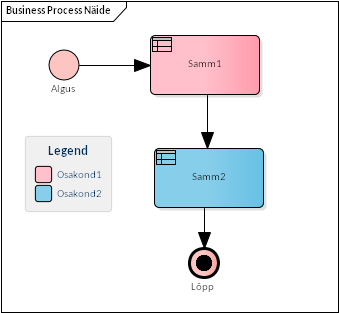
\includegraphics[width=\linewidth]{bpmn.png}
  \caption{Näide seoste kujutamisest eri kihtide vahel}
  \label{fig:bpmn}
\end{marginfigure}


Teie töö vastu tunnevad huvi järgmised osakonnad
\begin{description}
	\item[Teenuste osakond] Vastutab lõppkasutaja kogemuse ja interakstsiooni eest, nende hallata on ka deklaratsiooni vorm ning sellele kehtivad (ranged ja keerulised) reeglid
	\item[Kontrolli osakond] Vastutab kontrolli eest, mille kõik esitatud tuludeklaratsioonid läbivad
	\item[Arvelduste osakond] Hoolitseb, et toimuks riigi tulude arvestus ning et kodanikud oma enam-makstud tulumaksu pärast kontrolli tagasi saaksid
\end{description}

\section{Tulem}
\begin{marginfigure}%
  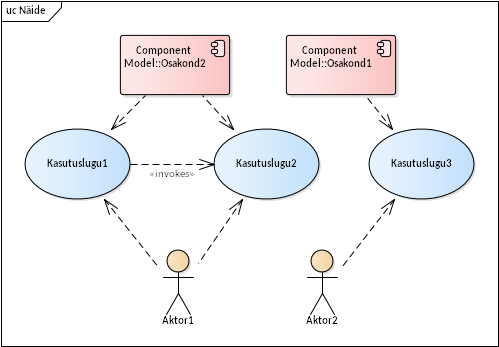
\includegraphics[width=\linewidth]{kasutuslood.png}
  \caption{Eri kihtide objektid samal diagrammil}
  \label{fig:uc}
\end{marginfigure}

Tulemis on esindatud järgmised kihid
\begin{description}
	\item[Organisatsioon] Mis organisatsiooni osad protsessis osalevad\sidenote{Vt. eelmist punkti minimaalse hulga osas, alati võib uusi üksusi lisada}
	\item[Äriprotsess] Millistest sammudest koosneb äriprotsess\sidenote{Piisab \enquote{happy day} stsenaariumist ja paarist alternatiivsest harust} ja kuidas on need sammud seotud organisatsiooniga
	\item[Kasutuslood] Mis kasutuslood\sidenote{Võib keskenduda peamisele väärtusprotsessile ja ignoreerida lisategevusi nagu kasutaja tuvastamine} realiseerivad millised protsessi sammud
	\item[Süsteemid] Millised süsteemid\sidenote{Linnaplaneerimise mõttes} leiduvad, millistesse tsoonidesse nad jagunevad ning mis kasutuslood puudutavad milliseid süsteeme?
	\item[Tehnilised komponendid] Millistest suurematest\sidenote{Klassidiagrammi tasemele ei ole vaja minna aga veebirakendus ja andmebaas võiksid olla markeeritud} komponentidest süsteemid koosnevad
\end{description}
\begin{marginfigure}%
  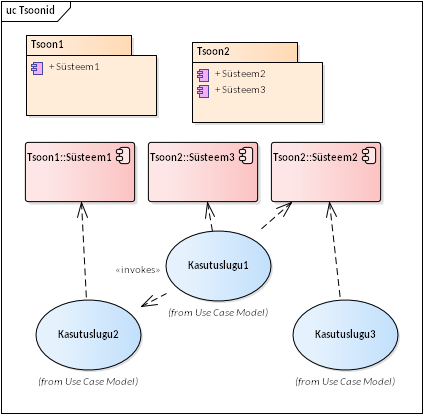
\includegraphics[width=\linewidth]{tsoonid.png}
  \caption{Eri kihtide objektid samal diagrammil}
  \label{fig:zone}
\end{marginfigure}

Eritüübiliste objektide vahelise seoste demonstreerimiseks võib kasutada millist iganes selge semantikaga vahendit. Peamised võimalused on
\begin{itemize}
	\item Seosed objektide vahel, nagu näidatud joonisel \ref{fig:uc}. 
	\item Värvid, nagu näidatud joonisel \ref{fig:bpmn}. Eri osakondade sammud on eri värvi. Sobilik, kui diagramm on keeruline ja seoste näitamine läheks liiale
	\item Sisalduvus paketis, nagu näidatud joonisel \ref{fig:zone}
\end{itemize}

Muidugi võib kasutada ka eri variantide kombinatsiooni, nagu joonisel \ref{fig:zone}



\bibliography{idu1321}
\bibliographystyle{plainnat}
\end{document}